\documentclass[a4paper,12pt]{article}

\usepackage[T2A]{fontenc} 
\usepackage[utf8]{inputenc}
\usepackage[english,russian]{babel}
\usepackage{listings}
\usepackage[dvips]{graphicx}
\usepackage{indentfirst}
\usepackage{color}
\usepackage{hyperref}
\usepackage{amsmath}
\usepackage{amssymb}
\usepackage{geometry}
\geometry{left=1.5cm}
\geometry{right=1.5cm}
\geometry{top=1cm}
\geometry{bottom=2cm}

\graphicspath{{images/}}

\begin{document}
\sloppy

\lstset{
	basicstyle=\small,
	stringstyle=\ttfamily,
	showstringspaces=false,
	columns=fixed,
	breaklines=true,
	numbers=right,
	numberstyle=\tiny
}

\newtheorem{Def}{Определение}[section]
\newtheorem{Th}{Теорема}
\newtheorem{Lem}[Th]{Лемма}
\newenvironment{Proof}
	{\par\noindent{\bf Доказательство.}}
	{\hfill$\scriptstyle\blacksquare$}
\newenvironment{Solution}
	{\par\noindent{\bf Решение.}}
	{\hfill$\scriptstyle\blacksquare$}


\begin{flushright}
	Кринкин М. Ю. группа 504 (SE)
\end{flushright}

\section{Домашнее задание 9}

\paragraph{Задание 1.} Сколькими способами можно выбрать из урны 5 шаров красного, синего, белого и черного цвета при условии, что красные шары выбираются по одному за раз, синего - по 4 за раз, белого - по 5 за раз и черного - по 3 за раз?

\begin{Solution}
Сопоставим выборам красных шаров производящую функцию:
\[
	f_1\left(x\right) = 1+x+x^2+x^3+x^4+...
\]
выборам синих шаров функцию:
\[
	f_2\left(x\right) = 1+x^4+x^8+x^{12}+...
\]
выборам белых шаров функцию:
\[
	f_3\left(x\right) = 1+x^5+x^{10}+x^{15}+...
\]
выборам черных сопоставим функцию:
\[
	f_4\left(x\right) = 1+x^3+x^6+x^9+..
\]
так как на коэффициент при $x^5$ не повлияют слогаемые со со степенями больше 5, ограничим производящие функции:
\[
	\begin{split}
		& f_1\left(x\right)=1+x+x^2+x^3+x^4+x^5 \\
		& f_2\left(x\right)=1+x^4 \\
		& f_3\left(x\right)=1+x^5 \\
		& f_4\left(x\right)=1+x^3
	\end{split}
\]
произведение приведенных функций:
\[
	\begin{split}
		&res\left(x\right) = 1+x+x^2+2\cdot x^3+3\cdot x^4+4\cdot x^5+3\cdot x^6+4\cdot x^7+5\cdot x^8+5\cdot x^9+4\cdot x^{10}+\\
		&+3\cdot x^{11}+4\cdot x^{12}+3\cdot x^{13}+2\cdot x^{14}+x^{15}+x^{16}+x^{17}
	\end{split}
\]
Таким образом возможны 4 способа:
\[
	\begin{split}
		& \{\{red,red,red,red,red\},\\
		& \{4 \times blue, red\},\\
		& \{5 \times white\},\\
		& \{3 \times black, red, red\}\}
	\end{split}
\]
\end{Solution}

\paragraph{Задание 2.} Сколько существует способов выбора 20 объектов из множества объектов пяти типов при условии, что количество объектов первого типа кратно пяти, второго - трем, объектов третьего типа следует выбирать не более четырех, четвертого - не менее трех, пятого - не более двух?

\begin{Solution}
Аналогично предыдущей задаче, с учетом всех ограничений получаем следующие производящие функции:
\[
	\begin{split}
		&f_1\left(x\right)=1+x^5+x^{10}+x^{15}+x^{20}\\
		&f_2\left(x\right)=1+x^3+x^6+x^9+x^{12}+x^{15}+x^{18}\\
		&f_3\left(x\right)=1+x+x^2+x^3+x^4\\
		&f_4\left(x\right)=\sum_{p=3}^{20} x^p\\
		&f_5\left(x\right)=1+x+x^2
	\end{split}
\]
результат произведения:
\[
	\begin{split}
		&res\left(x\right)=x^3+3\cdot x^4+6\cdot x^5+10\cdot x^6+15\cdot x^7+21\cdot x^8+28\cdot x^9+36\cdot x^{10}+\\
		&+45\cdot x^{11}+55\cdot x^{12}+66\cdot x^{13}+78\cdot x^{14}+91\cdot x^{15}+105\cdot x^{16}+120\cdot x^{17}+\\
		&+136\cdot x^{18}+153\cdot x^{19}+171\cdot x^{20}+...
	\end{split}
\]
Количество способов равно 171.
\end{Solution}

\paragraph{Задание 3.} Раньше в магазинах для взвешивания товаров использовались гири весом 1, 2, 3, 5 и 10 кг. С точки зрения комбинаторики более удачным был бы набор гирь в 1, 2, 4 и 8 кг - он бы, например, позволял единственным образом отвешивать любое число килограмм от 1 до 15. Вообще, имея по одной гире весом в 1, 2, 4, ..., $2^n$ кг, можно единственным образом получить любой вес от 1 до $2^{n-1}$ кг, кладя гири на одну чашу весов. Это утверждение очевидным образом доказывается с использованием записи такого числа в двоичной системе счисления.

\begin{itemize}
\item (a) Доказать тот же факт с использованием производящей функции.

\item (b) Из той же серии: доказать, что с помощью набора гирь в 1, 2, 2, 5, 10, 20, 50, 100, 200, 200, 500 мг можно составить любой вес, равный целому числу мг.
\end{itemize}

\begin{Solution}
Рассмотрим пункт (a). Суть доказать, что:
\[
	\prod_{i=0}^{n}\left(1+x^{2^i}\right)=\sum_{i=0}^{2^{n+1}-1}x^i
\]
покажем это по индукции. База индукции:
\[
	\left(1+x\right)\cdot\left(1+x^2\right)=1+x+x^2+x^3
\]
Индукционное предположение - пусть утверждение справедливо для $n$, покажем, что оно справедливо и для $n+1$:
\[
	\begin{split}
		&\left(1+x^{2^{n+1}}\right)\cdot\sum_{i=0}^{2^{n+1}-1}x^i = \sum_{i=0}^{2^{n+1}-1}x^i + x^{2^{n+1}}\cdot\sum_{i=0}^{2^{n+1}-1} = \sum_{i=0}^{2^{n+1}-1}x^i+\sum_{k=2^{n+1}}^{2\cdot 2^{n+1}-1}x^k = \sum_{i=0}^{2^{n+2}-1}x^i
	\end{split}
\]

Теперь рассмотрим пункт (b). Чисто технически доказательство сводится к произведению следующих производящих функций:
\[
	\begin{split}
		&f_1\left(x\right) = 1+x\\
		&f_2\left(x\right) = 1+x^2+x^4\\
		&f_3\left(x\right) = 1+x^5\\
		&f_4\left(x\right) = 1+x^{10}\\
		&f_5\left(x\right) = 1+x^{20}+x^{40}\\
		&f_6\left(x\right) = 1+x^{50}\\
		&f_7\left(x\right) = 1+x^{100}\\
		&f_8\left(x\right) = 1+x^{200}+x^{400}\\
		&f_9\left(x\right) = 1+x^{500}
	\end{split}
\]
Но учитывая, что максимальная степень в произведении $x^{1110}$, то проверять произведение руками будет довольно трудно, поэтому будем действовать подругому.
Произведение $f_1$, $f_2$ и $f_3$:
\[
	\left(1+x\right)\cdot\left(1+x^2+x^4\right)\cdot\left(1+x^5\right) = 1+x+x^2+x^4+2\cdot x^5+x^6+x^7+x^8+x^9+x^{10}
\]
таким образом произведение первых трех многочленов давет нам возможность получить все веса от 1 до 10. Нетрудно увидеть, что аналогичным образом произведение $f_4$, $f_5$ и $f_6$ позволяет получить все степени кратные 10 от 10 до 100, а так как произведение $f_1$, $f_2$ и $f_3$ позволяет получить любую степень до 10 включительно, то объединив все вместе, сможем получить все степени от 1 до 110. Аналогичным образом произведением функций $f_7$, $f_8$ и $f_9$ сможем получить все степени кратные 100 от 100 до 1000, то объединив с предыдущими результатами сможем получить все степени от 1 до 1110.

\end{Solution}

\paragraph{Задание 4.} С помощью диаграмм Ферре доказать, что:
\begin{itemize}
\item a) количество рабиений числа $2n + m$ на ровно $n+m$ слогаемых одинаково при любом $m \ge 0$; Чему оно равно?

\item б) количество разбиений числа $n$ на четные слгаемые равно количеству разбиений, в котором любое из чисел (т. е. частей разбиения) входит четное число раз.

\item в) количество разбиений числа $n-m$ ровно на $k-1$ частей, любое из которых меньше или равно $m$, равно количеству разбиений числа $n-k$ ровно на $m-1$ частей, любое из которых меньше или равно $k$.

\item г) количество разбиений числа $n$ на $k$ частей равно количеству разбиений числа $n + {k\left(k-1\right)}/2$ ровно на $k$ неравных частей.
\end{itemize}

\begin{Solution}
Рассмотрим пункт а). Так как число $2n + m$ разбито ровно на $n+m$ слогаемых, в каждой диаграмме Ферре будет столбце из $n+m$ точек, удалим этот столбец и получим все разбиения числа $n$. Возможно и обратное приобразование, которое разбиению числа $n$ сопоставляет разбиение числа $2n + m$ ровно на $n+m$ слогаемых, такое преобразование осуществляется добавлением столбца из $n+m$ точек.

\begin{figure}[h]
\begin{center}
\noindent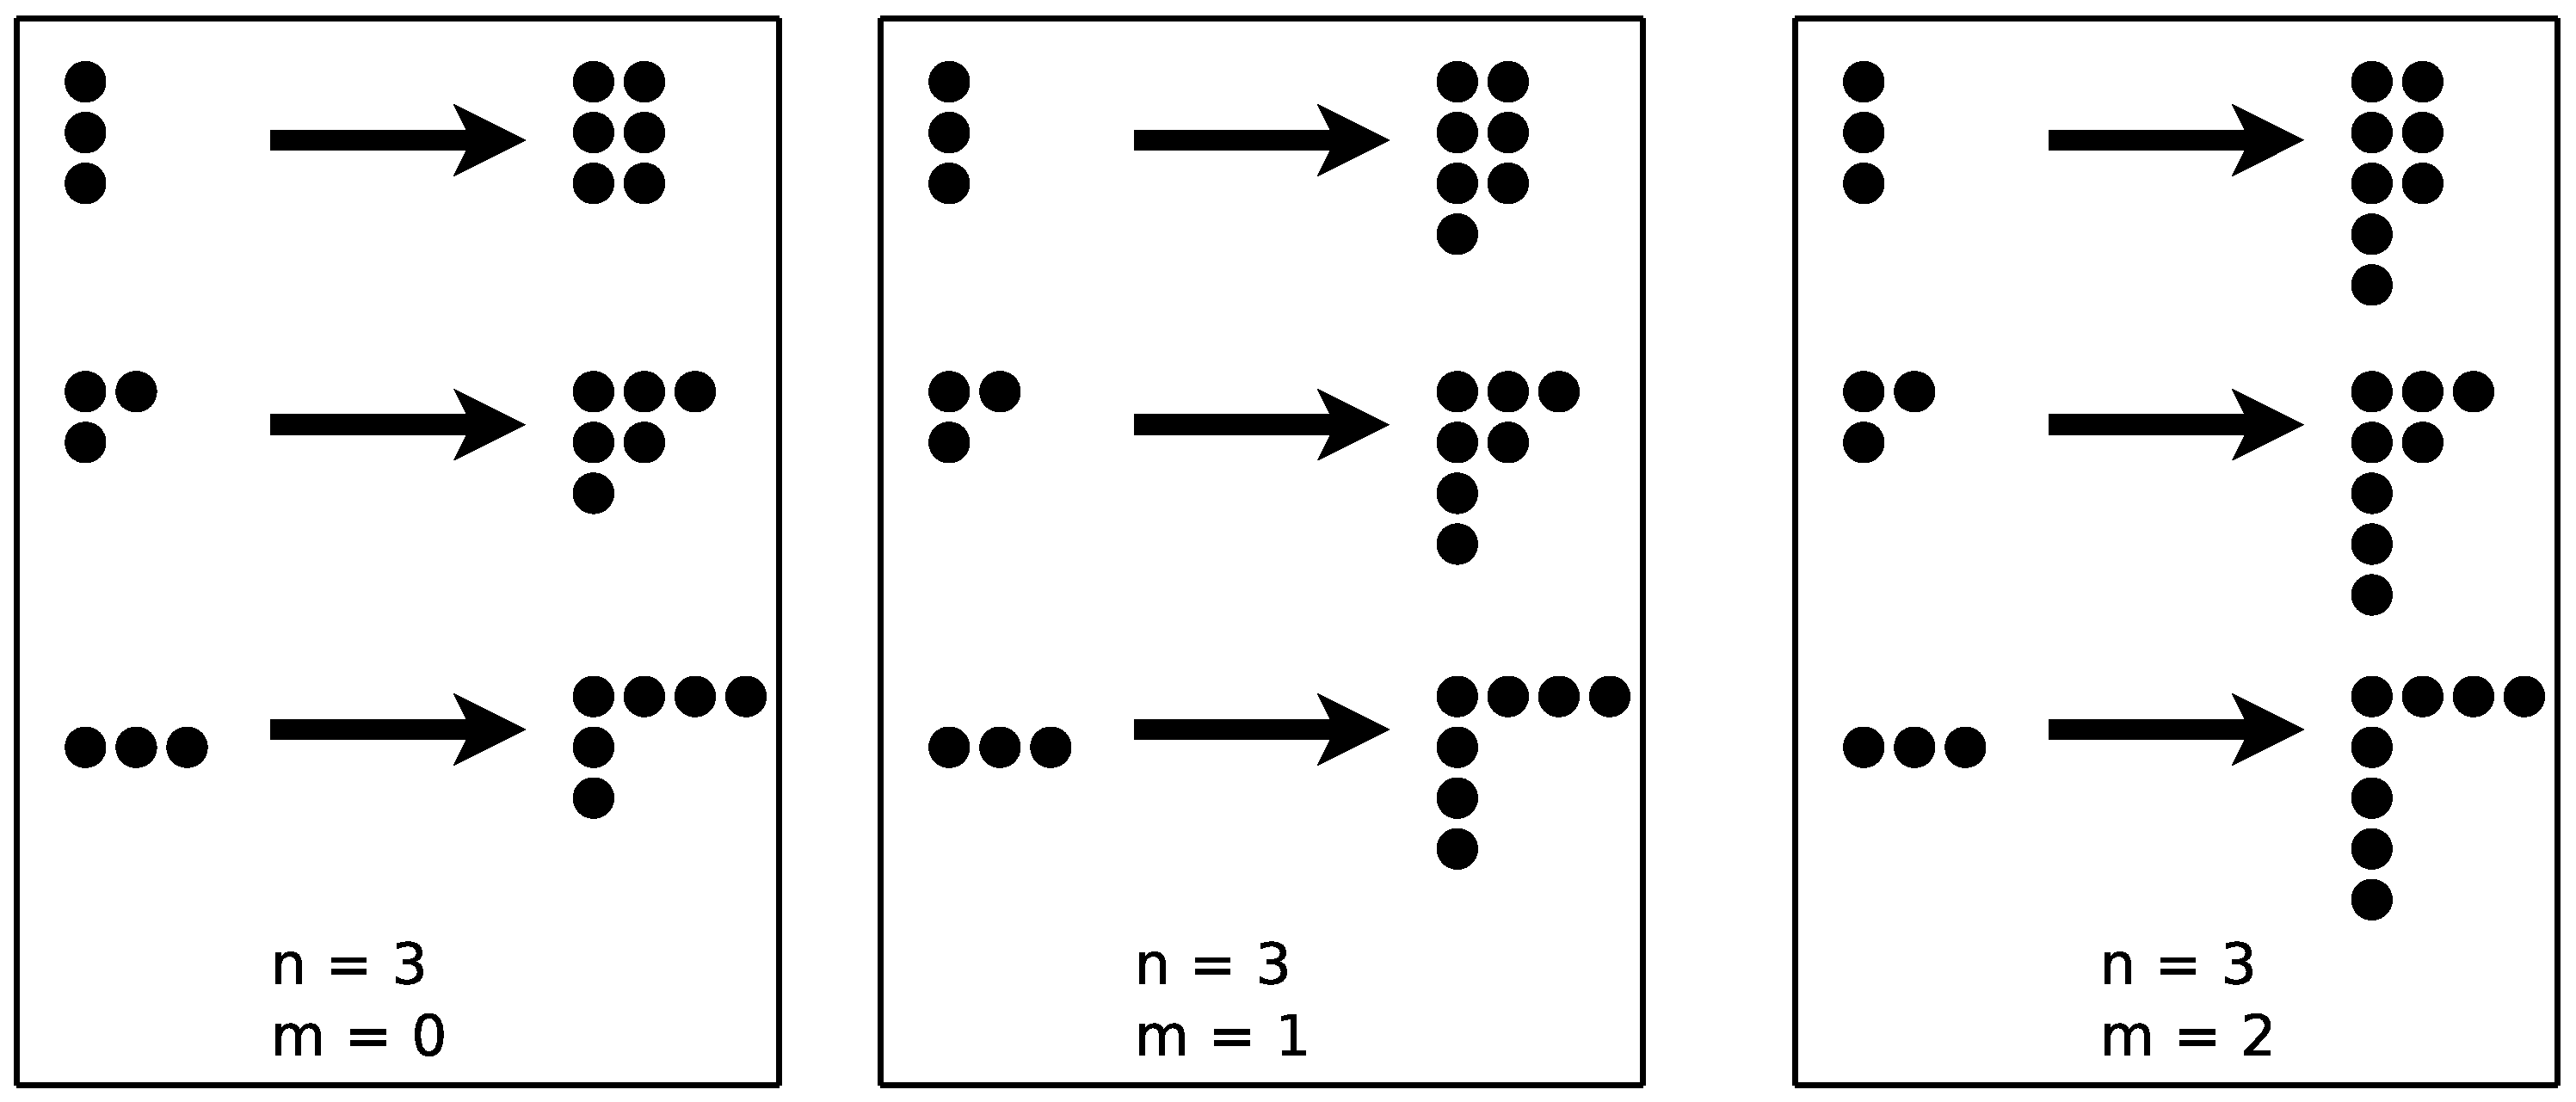
\includegraphics[width=0.4\linewidth]{ferre1}
\caption{Пункт а}
\label{img::ferre1}
\end{center}
\end{figure}
Если посмотреть на рисунок \ref{img::ferre1}, то видно, что от $m$ преобразование не зависит, так как для различных $m$ диаграммы различаются лишь <<хвостом>> из $m$ единичных строк, а всего таких разбиений $P\left(n\right)$.

Теперь рассмотрим пункт б). В этом задании достаточно транспонировать диаграмму Ферре, так как как если каждое слогаемое в разбиении $n$ четно, то либо они все одинаковы, и в этом случае, получаем транспонированием разбиение $n$ на четное число равных слогаемых. Если же слогаемые в разбиении $n$ различны, т. к. все они четны, то и разности между ними четны, значит в исходной диаграмме будет четное число столбцов равной высоты, которые при транспонировании перейдут в строки равной длинны. Пример на рисунке \ref{img::ferre2}.

\begin{figure}[h]
\begin{center}
\noindent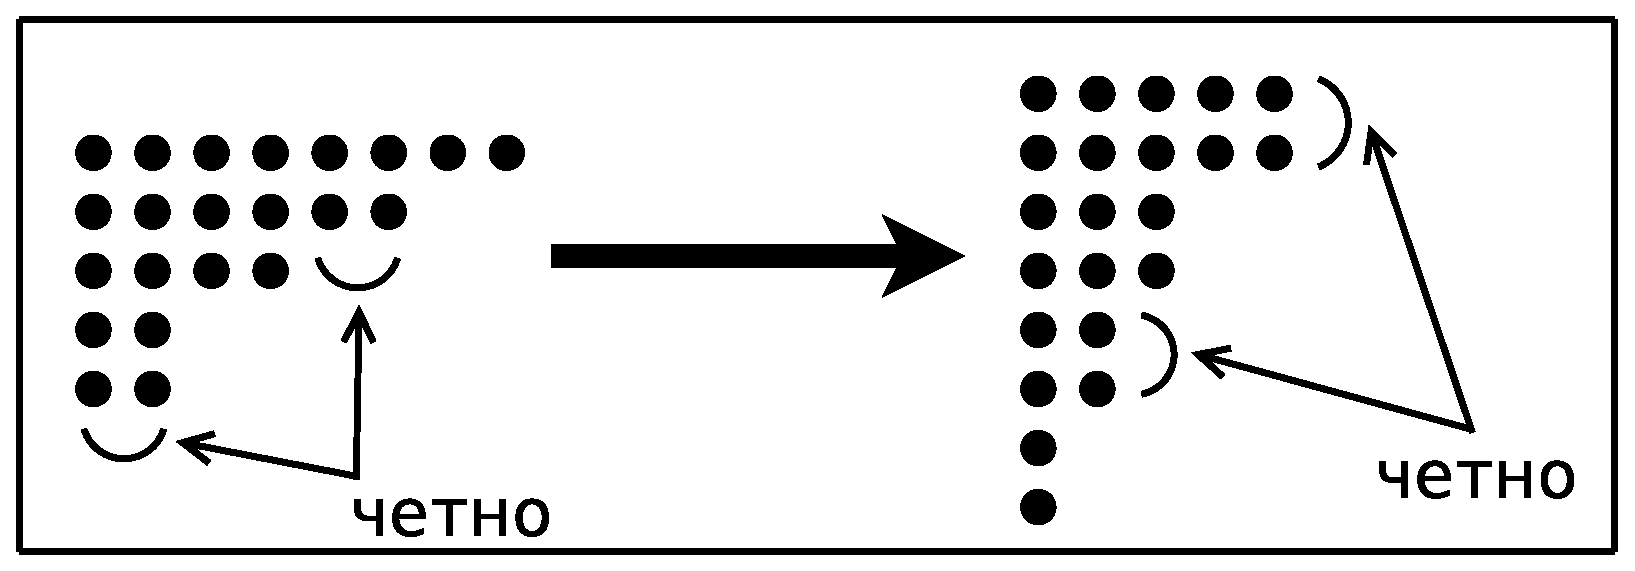
\includegraphics[width=0.4\linewidth]{ferre2}
\end{center}
\caption{Пункт б}
\label{img::ferre2}
\end{figure}

Теперь рассмотрим пункт в). Если $m > k$, тогда $n-m < n-k$, и в этом случае действуем следующим образом:
\begin{enumerate}
\item Выделяем последний столбец и переносим точки из него в строку. Таким образом переходим от диаграммы с $m$ столбцами к диаграмме с $m-1$ столбцами.

\item Добавляем к диаграмме $m-k$ точек, заполняя строки поочередно пока не закончатся $m-k$ точек, так чтобы длина строк не превышала $m-1$. (см рисунок \ref{img::ferre3}).

\item Транспониуем диаграмму. Таким образом получаем диаграмму с $m-1$ строкой и длинной строки не более чем $k$, так как на предыдущем шаге не может быть добавлено более $1$ строки.
\end{enumerate}

\begin{figure}[h]
\begin{center}
\noindent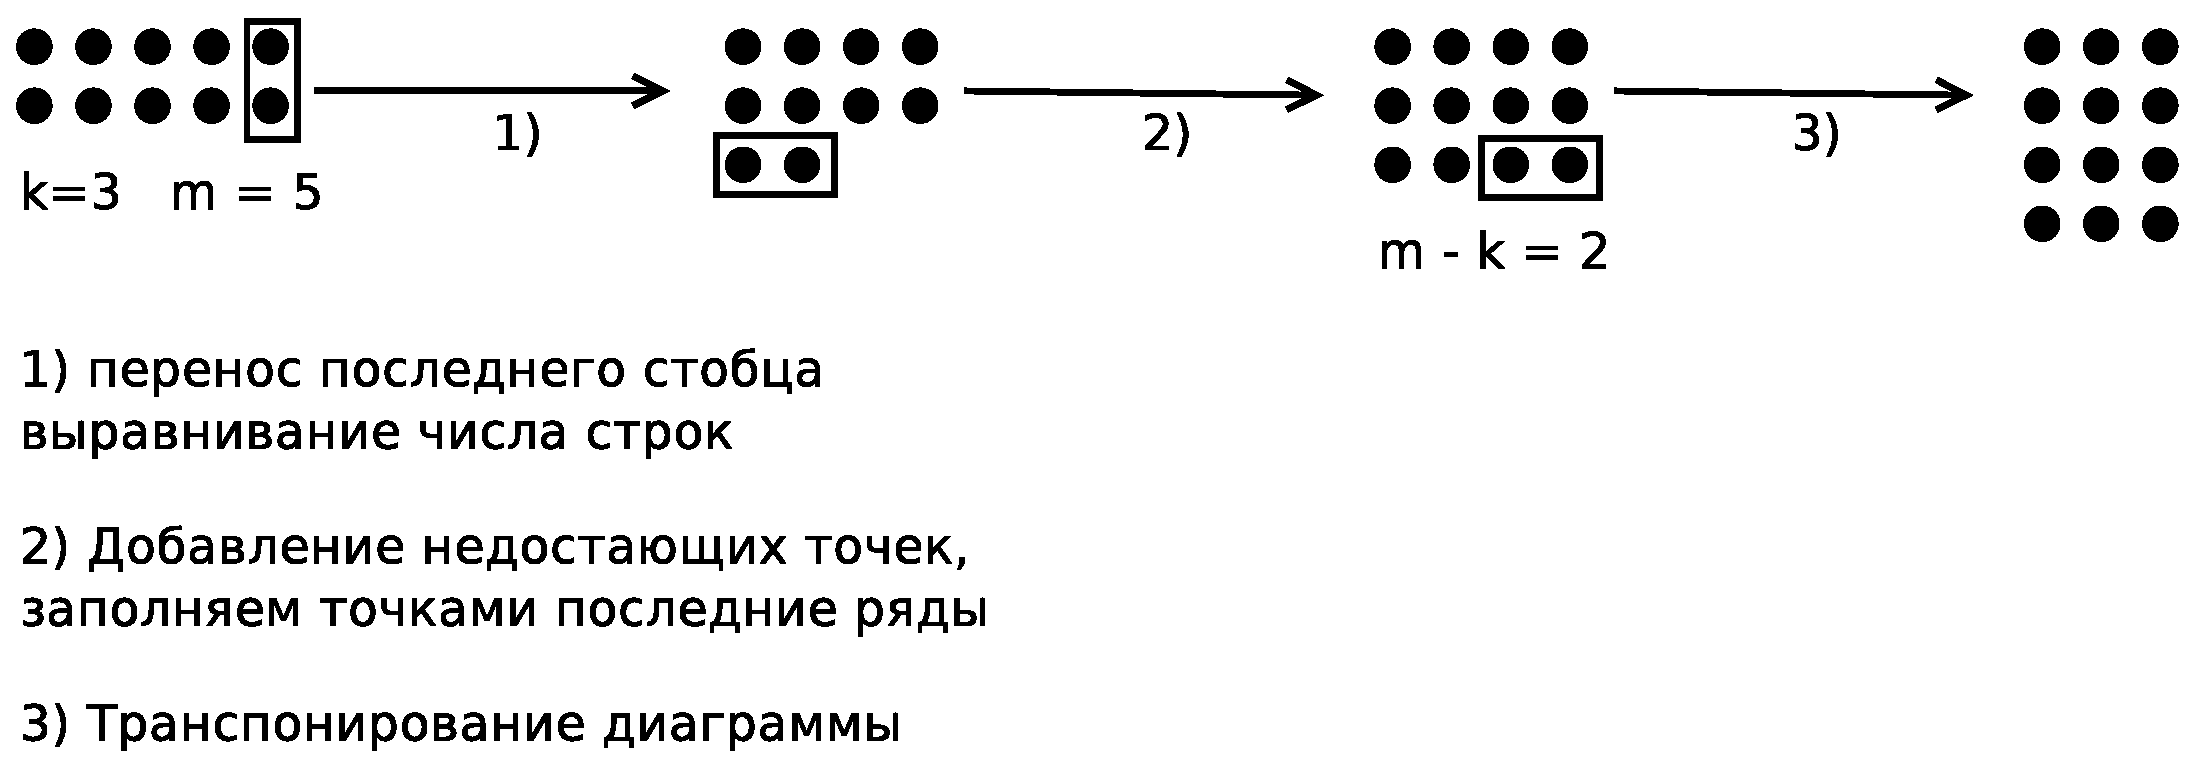
\includegraphics[width=0.4\linewidth]{ferre3}
\end{center}
\caption{Пункт в, $m>k$}
\label{img::ferre3}
\end{figure}

Если же имеем обратную ситуацию, то выполняем все действия в точности наоборот (то есть делаем обратное преобразование), см. рисунок \ref{img::ferre4}

\begin{figure}[h]
\begin{center}
\noindent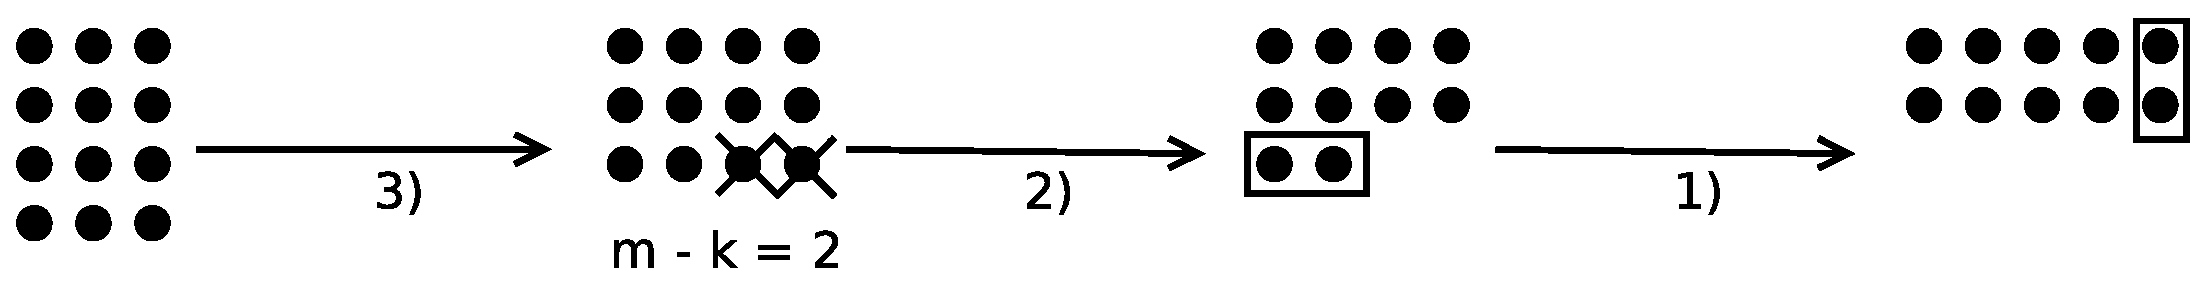
\includegraphics[width=0.4\linewidth]{ferre4}
\end{center}
\caption{Пункт в, $m\le k$}
\label{img::ferre4}
\end{figure}

Ну и наконец пункт г). Эта задача полностью эквивалентна задаче, которую мы решали в аудитории, с той лишь разницей, что изначально имеем диаграмму для разбиения числа $n$ ровно на $k$ частей, поэтому для того, чтобы все строки в соответствующей диаграмме были различны достаточно добавить треугольник из ${k \left(k-1\right)}/2$ точек как показано на рисунке \ref{img::ferre5}

\begin{figure}[h]
\begin{center}
\noindent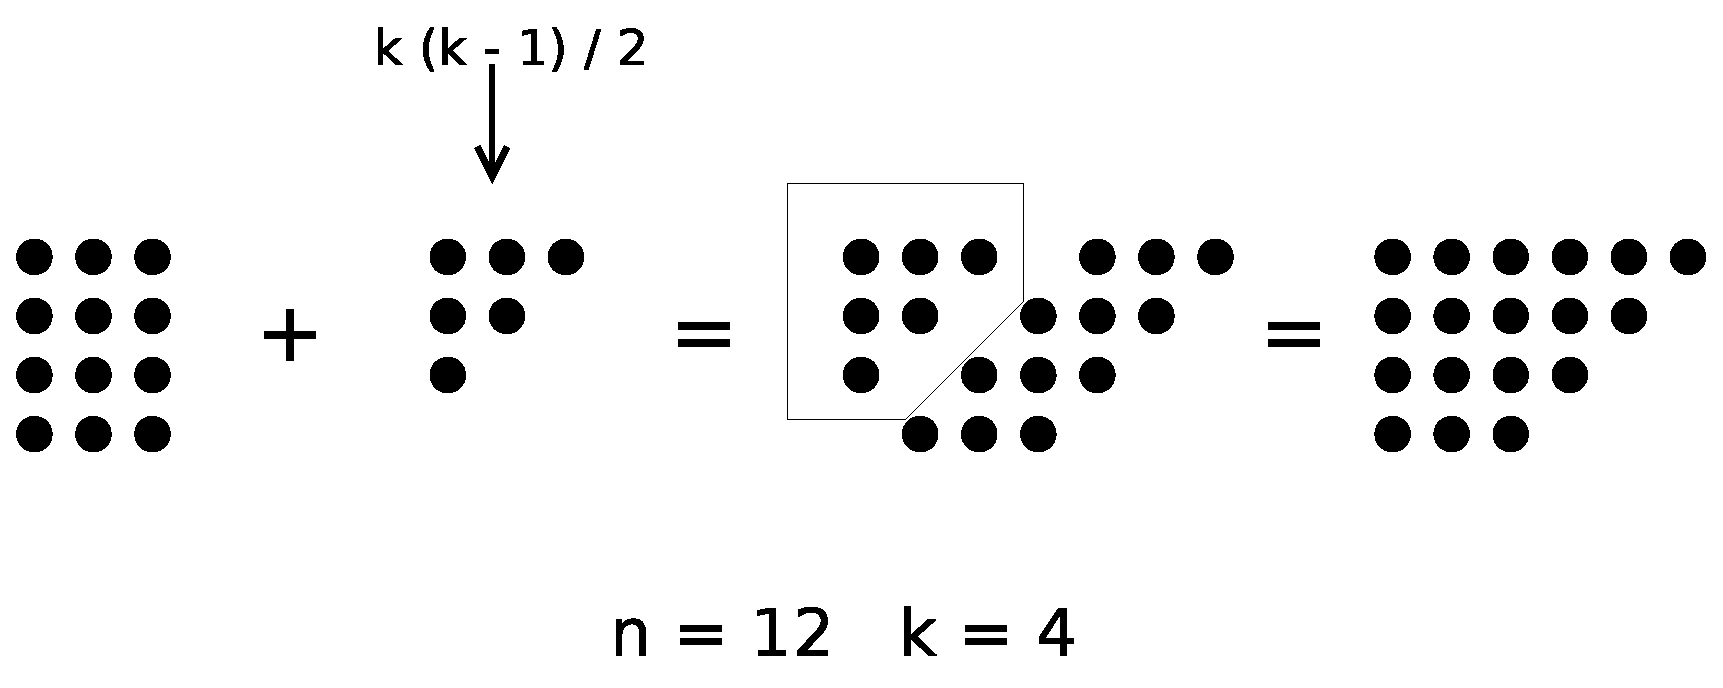
\includegraphics[width=0.4\linewidth]{ferre5}
\end{center}
\caption{Пункт г}
\label{img::ferre5}
\end{figure}

\end{Solution}

\paragraph{Задание 5.} С использованием производящей функции показать, что
\begin{itemize}
\item а)
\[
	p_2\left(k\right) = \lfloor\frac{n}{2}\rfloor
\]
где $\lfloor k \rfloor$ - ближайшее целое к числу $k$, меньшее или равное $k$

\item б)
\[
	p_3\left(n\right) = \{\frac{n^2}{12}\}
\]
где $\{k\}$ - ближайшее целое к числу $k$.

\item в)
\[
	p_k\left(n\right) \sim \frac{n^{k-1}}{k! \left(k-1\right)!}
\]
где символ $p \sim k$ означает, что число $p$ по порядку равно $k$ при больших значениях $k$.
\end{itemize}

\begin{Solution}
Рассмотрим пункт a). Для чисел $p_k\left(n\right)$ известно рекуррентное соотношение:
\[
	p_k\left(n\right) = p_{k-1}\left(n-1\right) + p_k\left(n-k\right)
\]
и начальные условия можно задать так:
\[
	\begin{split}
		&p_k\left(k\right) = 1\\
		&p_1\left(n\right) = 1
	\end{split}
\]
Построим производящую функцию для $k = 2$:
\[
	\begin{split}
		&\sum_{n=0}^{\infty} x^{n+2} p_2\left(n+2\right) = 1 + \sum_{n=0}^{\infty}x^{n+2} p_2\left(n\right) \Leftrightarrow \\
		&\Leftrightarrow f\left(x\right) = \frac{x^2}{1-x} + x^2 f\left(x\right) \Leftrightarrow f\left(x\right) = \frac{x^2}{\left(1-x\right)\left(1-x^2\right)}
	\end{split}
\]
Откуда получаем разложив в ряд:
\[
	p_2\left(n\right) = \frac{\left(-1\right)^{n-2}}{4} + \frac{n-1}{2} + \frac{1}{4}
\]
а теперь рассматриваем случаи:
\begin{enumerate}
\item $n = 2k + 1$, тогда $p_2\left(n\right) = -\frac{1}{4} + \frac{2k}{2} + \frac{1}{4} = k$

\item $n = 2k$, тогда $p_2\left(n\right) = \frac{1}{4} + \frac{2k}{2} - \frac{1}{2} + \frac{1}{4} = k$
\end{enumerate}

Рассмотрим пункт в). Для начала рассмотрим несколько начальных значений числа $p_3\left(n\right)$:

\begin{tabular}[t]{|c|c|c|c|c|c|c|c|}
\hline
$n$                 & 0 & 1 & 2 & 3 & 4 & 5 & 6 \\
\hline
$p_3\left(n\right)$ & 0 & 0 & 0 & 1 & 1 & 2 & 3 \\
\hline
\end{tabular}

Для них очевидно условие выполняется, далее воспользуемся рекуррентной формулой, для доказательства по индукии:
\[
	\begin{split}
		&p_3\left(n+3\right) = p_2\left(n+2\right) + p_3\left(n\right) \Leftrightarrow \\
		&\Leftrightarrow p_3\left(n+3\right) = \lfloor \frac{n+2}{2} \rfloor + \{\frac{n^2}{12}\}
	\end{split}
\]

Рассмотрим варианты возможных условий на $n$:
\begin{itemize}
\item $n=6k$, тогда справа имеем $\lfloor \frac{6k + 2}{2} \rfloor + \{\frac{36 k^2}{12}\} = 3k + 1 + 3 k^2$, а слева, по доказываемой формуле $\{\frac{36 k^2 + 36 k + 9}{12}\} = 3 k^2 + 3k + 1$

\item $n=6k+1$, тогда справа имеем $\lfloor \frac{6k + 3}{2} \rfloor + \{\frac{36 k^2 + 12k + 1}{12}\} = 3k + 1 + 3 k^2 + k$, слева $\{\frac{36 k^2 + 48 k + 16}{12}\} = 3 k^2 + 4k + 1$

\item $n=6k+2$, справа $\lfloor \frac{6k + 4}{2} \rfloor + \{\frac{36 k^2 + 24 k + 4}{12}\} = 3k + 2 + 3 k^2 + 2k$, слева $\{\frac{36 k^2 + 60 k + 25}{12}\} = 3 k^2 + 5k + 2$

\item $n=6k+3$, справа $\lfloor \frac{6k + 5}{2} \rfloor + \{\frac{36 k^2 + 36 k + 9}{12}\} = 3k + 2 + 3 k^2 + 3 k + 1$, слева $\{\frac{36 k^2 + 72 k + 36}{12}\} = 3 k^2 + 6 k + 3$

\item $n=6k+4$, справа $\lfloor \frac{6k + 6}{2} \rfloor + \{\frac{36 k^2 + 48 k + 16}{12}\} = 3k + 3 + 3 k^2 + 4k + 1$, слева $\{\frac{36 k^2 + 84 k + 49}{12}\} = 3 k^2 + 7 k + 4$

\item $n=6k+5$, справа $\lfloor \frac{6k + 7}{2} \rfloor + \{\frac{36 k^2 + 60 k + 25}{12}\} = 3k + 3 + 3 k^2 + 5 k + 2$, слева $\{\frac{36 k^2 + 96 k + 64}{12}\} = 3 k^2 + 8 k + 5$
\end{itemize}
т. е. по индукции получаем, что утверждение справедливо и для больших $n$.

Теперь докажем утверждение в). Рассмотрим сначала оценку на верхнюю границу числа $p_k\left(n\right)$. $p_k\left(n\right)$ равно количеству разбиений числа $n + \frac{k\left(k-1\right)}{2}$ на различные слогаемые, но каждое такое слогаемое дает $k!$ слогаемых с учетем порядка. Всего упорядоченных разбиений $\binom{n+\frac{k\left(k-1\right)}{2} - 1}{k-1}$, так как в это число входят еще и разбиения с повторяющимися слогаемыми, то
\[
	p_k\left(n\right) < \frac{1}{k!} \binom{n+\frac{k\left(k-1\right)}{2} - 1}{k-1}
\]

Теперь рассмотрим оценку на нижнюю границу числа $p_k\left(n\right)$. Количество упорядоченных разбиений числа $n$ на $k$ слогаемых, опять же, $\binom{n-1}{k-1}$. Т. к. каждому неупорядоченному разбиению числа $n$ на $k$ слогаемых соответствует не более $k!$ упорядоченных разбиений, то $\frac{1}{k!} \binom{n-1}{k-1} < p_k\left(n\right)$. Вместе получаем:
\[
	\frac{1}{k!} \binom{n-1}{k-1} < p_k\left(n\right) < \frac{1}{k!} \binom{n + \frac{k\left(k-1\right)}{2} -1}{k-1}
\]

Теперь раскрываем $\frac{1}{k!}\binom{n - 1}{k - 1}$:
\[
	\frac{1}{k!} \binom{n-1}{k-1} = \frac{\left(n-1\right)\left(n-2\right)...\left(n-k+1\right)}{k!\left(k-1\right)!} = \frac{n^{k-1}}{k!\left(k-1\right)!} + P_{k-2}\left(n\right)
\]
где $P_{k-2}\left(n\right)$ - многочлен степени не выше $k-2$ от $n$

Аналогичное рассуждение справедливо и для $\frac{1}{k!} \binom{n+\frac{k\left(k-1\right)}{2}-1}{k-1}$.
\end{Solution}

\paragraph{Задание 6.} Пусть $p\left(n;k,m-k\right)$ есть количество разбиений $n$ на не более чем $k$ слагаемых, каждое из которых меньше или равно $m-k$.
\begin{itemize}
\item а) Показать, что эти числа обладают следующими очевидными свойствами:
\[
	\begin{split}
		&p\left(n;k,m-k\right) = 0, \text{ если } n > k\cdot \left(m-k\right) \\
		&p\left(n;k,m-k\right) = 1, \text{ если } n = k\cdot \left(m-k\right) \\
		&p\left(n;k,m-k\right) = p\left(n;m-k,k\right)
	\end{split}
\]

\item б) Доказать, что
\[
	\binom{m}{k}_q = \binom{m-1}{k}_q + q^{m-k}\binom{m-1}{k-1}_q = q^k \binom{m-1}{k}_q + \binom{m-1}{k-1}_q
\]
и построить с помощью этого соотношения т. н. треугольник Паскаля.

\item в) С использованием предыдущих результатов определить, сколько существует диаграмм Ферре, которые можно разместить в прямоугольнике $k\cdot \left(m-k\right)$.

\item г) Получить ответ на предыдущий вопрос, используя интерпритацию разбиения числа $n$ как решения уравнения
\[
	\begin{split}
		&x_1 + x_2 + ... + x_k = n \\
		&x_1 \ge x_2 \ge x_3 \ge ... \ge x_k \ge 0
	\end{split}
\]
\end{itemize}

\begin{Solution}
Пункт а). Разбиениям, количество которых обозначено как $p\left(n;k,m-k\right)$, можно сопоставить диаграммы Ферре, все эти диаграммы имеют не больше $k$ строк и какждая строка не длиенне $m-k$, т. е. вписаны в прямоугольник $k \times m-k$.

Исходя из описанной интерпритации очевидно, что нельзя вписать в прямоугольник $k \times m-k$ диаграмму Ферре для разбиения числа $n > k \cdot \left(m-k\right)$, поэтому первое утверждение очевидно.

Второе утверждение также очевидно, так как существует всего одна диаграмма Ферре с $k \cdot \left(m-k\right)$ точками входящая в прямоугольник $k \cdot \left(m-k\right)$, а именно разбиение $n$ на $k$ равных слогаемых по $m-k$ каждое.

Третье утверждение соответсвует просто транспонированию диаграммы Ферре, поэтому также очевидно.

Пункт б). Докажем сначала второе равенство. Рассмотрим диаграммы Ферре вписанные в прямоугольник с $k$ строками и $m-k$ столбцами. Рассмотрим два возможных случая:
\begin{enumerate}
\item Верхняя строка заполнена. Тогда удалим эту строку, если в исходной диаграмме было $N$ точек, то в новой будет $N-k$, а кроме того в ней $k-1$ строка, каждая из которых длинны не более $m-k$. Обратное преобразование также справедливо, т. е. преобразование взаимооднозначно.

\item Верхняя строка $<m-k$. Но тогда исходная диаграмма умещается в прямоугольник $k \times m-k-1$.
\end{enumerate}

Получаем соотношение:
\[
	p\left(N;k,m-k\right) = p\left(N-k;k-1,m-k\right) + p\left(N;k,m-k-1\right)
\]
Умножим обе его части на $q^N$ и просуммируем по всем $N$:
\[
	\begin{split}
		& \sum_{N=0}^{\infty} q^N\left(N;k,m-k\right) = q^k \sum_{N=0}^{\infty} q^{N-k}p\left(N-k;k-1,m-k\right) + \sum_{N=0}^{\infty} q^N p\left(N;k,m-k-1\right) \Rightarrow \\
		& \Rightarrow \binom{m}{k}_q = q^k\binom{m-1}{k}_q + \binom{m-1}{k-1}_q
	\end{split}
\]

Если в рассуждении поменять местами $k$ и $m-k$, то получим первое равенство.

Трегольник Паскаля для $\binom{m}{k}_q$:
\[
	\begin{matrix}
		&&&&& 1\\
		&&&& 1 && 1\\
		&&& 1 && 1+q && 1\\
		&& 1 && q^2+q+1 && q^2+q+1 && 1\\
		& 1 && q^3+q^2+q+1 && q^4+q^3+2\cdot q^2+q+1 && q^3+q^2+q+1 && 1\\
	\end{matrix}
\]

Пункт в). Если подставить вместо $q$ единицу мы с одной стороны получаем требуемую сумму по всем $p\left(n;k,m-k\right)$, а с другой при $q = 1$ полученное выше соотношение в точности соотношение для биномиальных коэффициентов и для малых значений $n$ легко проверить, что они совпадают с биномиальными коэффициентами, таким образом требуемое искомое число $\binom{m}{k}$.

Пункт г). Если интерпритировать задачу как разбиение числа $n$, то задача сводится к выбору значений $k$ переменных, каждое из которых лежит в диапазоне $[0;m-k]$, т. е. всего $m-k+1$ возможных значений, причем возможны повторения:
\[
	\left(\binom{m-k+1}{k}\right) = \binom{m}{k}
\]
\end{Solution}

\end{document}
